\subsection{Sustitución}
La idea es tomar una parte de una formula y sustituirla por algo equivalente que sea más manejable. Definamos de forma rigurosa el concepto. 

\begin{figure}[h]
\centering
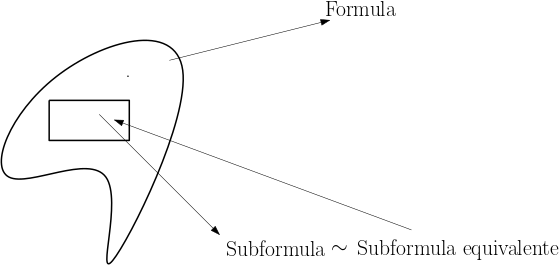
\includegraphics[width=8cm]{susti}
\end{figure}

\begin{definition} Sean $\varphi, \, \psi \in \p$ y $p \in \mbox{SP}$, se denota
\[ \psi[\varphi/p] \]
a sustituir en la fórmula $\psi$ las apariciones de $p$ por $\varphi$.
\end{definition}

El esquema queda

\begin{figure}[h]
\centering
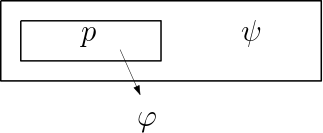
\includegraphics[width=6cm]{esq}
\end{figure}

